\subsection*{ตัวอย่างชุดข้อมูลสำหรับการทดสอบโมเดลปัญญาประดิษฐ์ในการตรวจจับภาพบุคคล}
\begin{figure}[!ht]
    \centering
   \begin{subfigure}[b]{0.55\linewidth}
      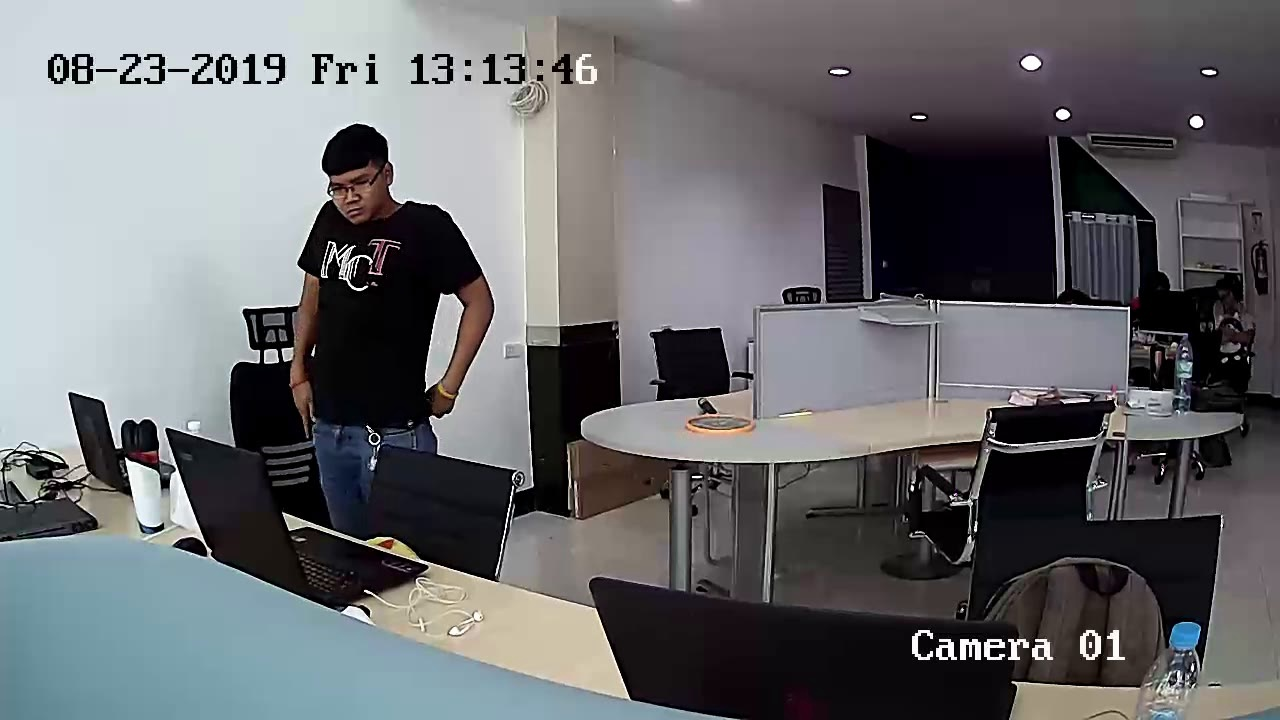
\includegraphics[width=\linewidth]{appendix/images/3.jpg}
    \end{subfigure}
    \begin{subfigure}[b]{0.55\linewidth}
      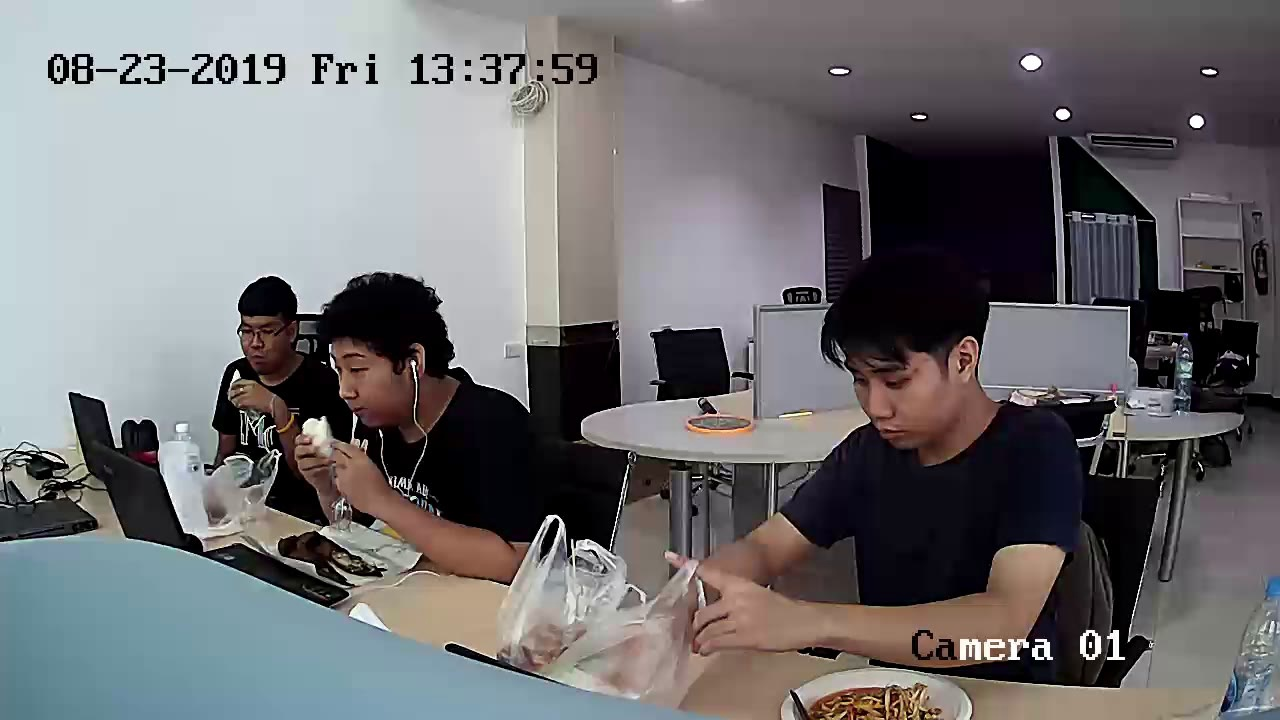
\includegraphics[width=\linewidth]{appendix/images/5.jpg}
    \end{subfigure}
    \begin{subfigure}[b]{0.55\linewidth}
      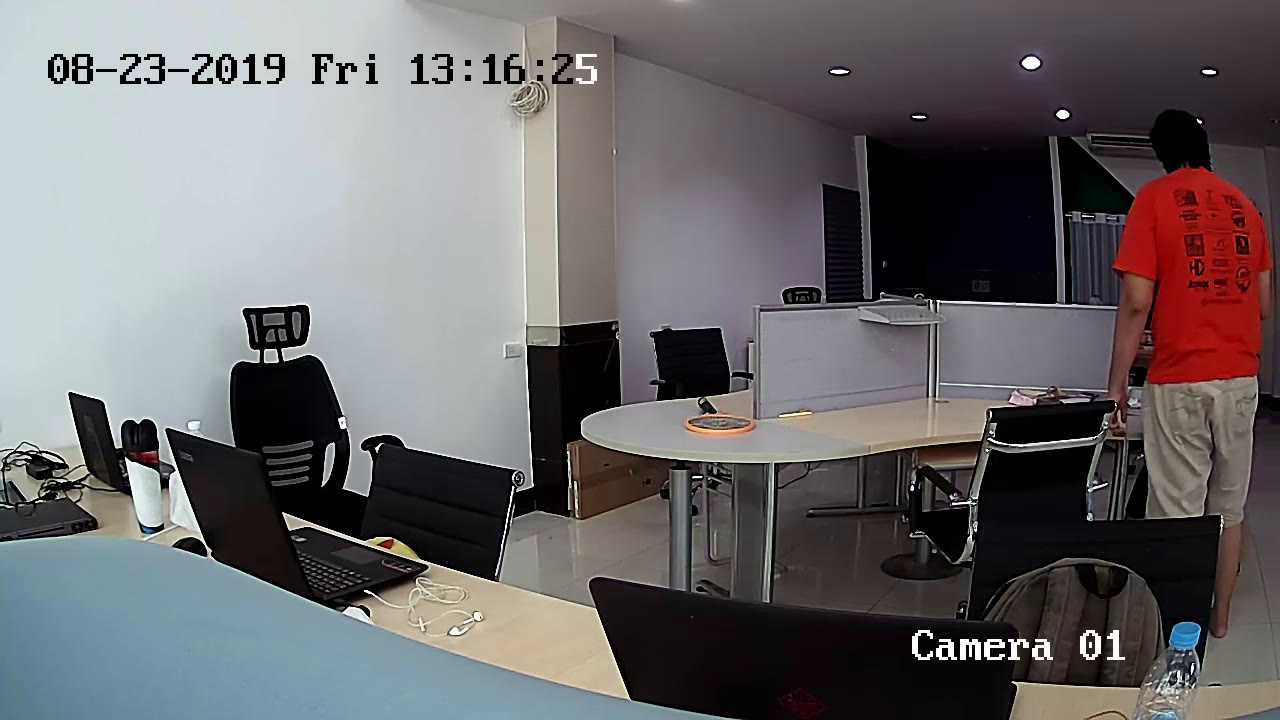
\includegraphics[width=\linewidth]{appendix/images/8.jpg}
    \end{subfigure}
    \begin{subfigure}[b]{0.55\linewidth}
      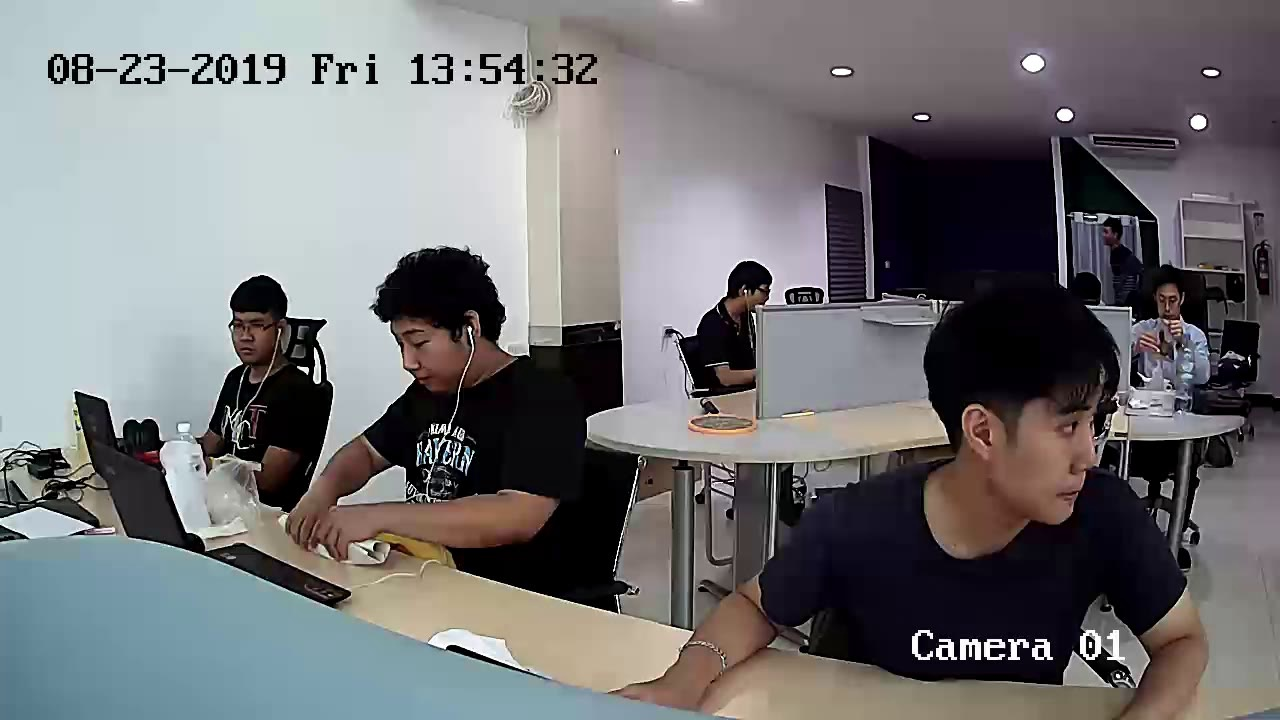
\includegraphics[width=\linewidth]{appendix/images/17.jpg}
    \end{subfigure}
    \caption{ตัวอย่างชุดข้อมูลสำหรับการทดสอบโมเดลปัญญาประดิษฐ์ในการตรวจจับภาพบุคค}
    \label{fig:result_track}
  \end{figure}

\subsection*{ตัวอย่างชุดข้อมูลสำหรับการสร้างโมเดลในหมวดหมู่ การตอบรับโทรศัพท์}
\begin{figure}[!ht]
    \centering
   \begin{subfigure}[b]{0.45\linewidth}
      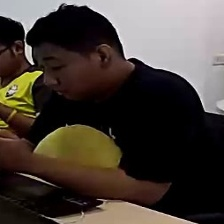
\includegraphics[width=\linewidth]{appendix/answer_phone/000_CXS0_D0_000038.jpg}
    \end{subfigure}
    \begin{subfigure}[b]{0.45\linewidth}
      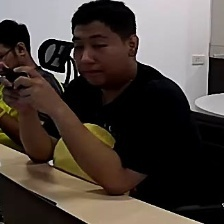
\includegraphics[width=\linewidth]{appendix/answer_phone/000_CXS0_D0_001102.jpg}
    \end{subfigure}
    \begin{subfigure}[b]{0.45\linewidth}
      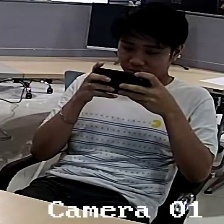
\includegraphics[width=\linewidth]{appendix/answer_phone/000_CXS0_D0_001293.jpg}
    \end{subfigure}
    \begin{subfigure}[b]{0.45\linewidth}
      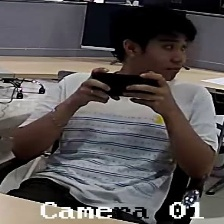
\includegraphics[width=\linewidth]{appendix/answer_phone/000_CXS0_D0_001791.jpg}
    \end{subfigure}
    \begin{subfigure}[b]{0.45\linewidth}
      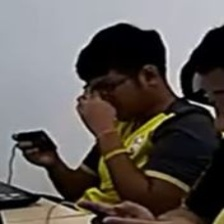
\includegraphics[width=\linewidth]{appendix/answer_phone/000_CXS0_D0_001792.jpg}
    \end{subfigure}
    \begin{subfigure}[b]{0.45\linewidth}
      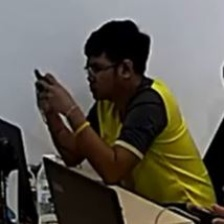
\includegraphics[width=\linewidth]{appendix/answer_phone/000_CXS0_D0_001793.jpg}
    \end{subfigure}
    \caption{ตัวอย่างชุดข้อมูลในหมวดหมู่การตอบรับโทรศัพท์}
    \label{fig:result_track}
  \end{figure}

\clearpage
\subsection*{ตัวอย่างชุดข้อมูลสำหรับการสร้างโมเดลในหมวดหมู่ การกิน }
\begin{figure}[!ht]
    \centering
   \begin{subfigure}[b]{0.45\linewidth}
      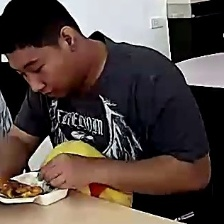
\includegraphics[width=\linewidth]{appendix/eat/000_CXS1_D0_000455.jpg}
    \end{subfigure}
    \begin{subfigure}[b]{0.45\linewidth}
      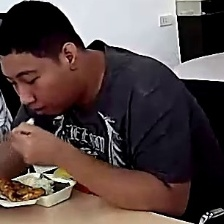
\includegraphics[width=\linewidth]{appendix/eat/000_CXS1_D0_001035.jpg}
    \end{subfigure}
    \begin{subfigure}[b]{0.45\linewidth}
      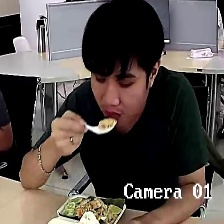
\includegraphics[width=\linewidth]{appendix/eat/001_CXS1_D0_001176.jpg}
    \end{subfigure}
    \begin{subfigure}[b]{0.45\linewidth}
      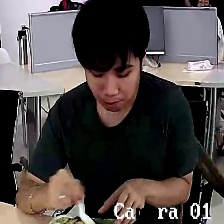
\includegraphics[width=\linewidth]{appendix/eat/001_CXS1_D0_001318.jpg}
    \end{subfigure}
    \begin{subfigure}[b]{0.45\linewidth}
      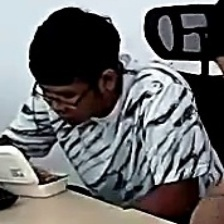
\includegraphics[width=\linewidth]{appendix/eat/001_CXS1_D0_001110.jpg}
    \end{subfigure}
    \begin{subfigure}[b]{0.45\linewidth}
      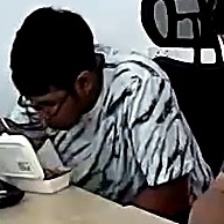
\includegraphics[width=\linewidth]{appendix/eat/001_CXS1_D0_001397.jpg}
    \end{subfigure}
    \caption{ตัวอย่างชุดข้อมูลในหมวดหมู่การกิน}
    \label{fig:result_track}
  \end{figure}

\clearpage
\subsection*{ตัวอย่างชุดข้อมูลสำหรับการสร้างโมเดลในหมวดหมู่ การนั่ง }
\begin{figure}[!ht]
    \centering
   \begin{subfigure}[b]{0.45\linewidth}
      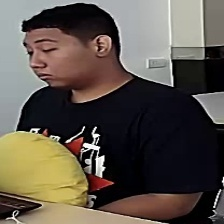
\includegraphics[width=\linewidth]{appendix/sit/000_CXS0_D0_003661.jpg}
    \end{subfigure}
    \begin{subfigure}[b]{0.45\linewidth}
      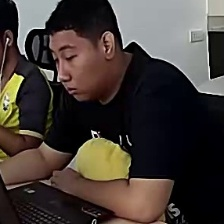
\includegraphics[width=\linewidth]{appendix/sit/000_CXS0_D0_006682.jpg}
    \end{subfigure}
    \begin{subfigure}[b]{0.45\linewidth}
      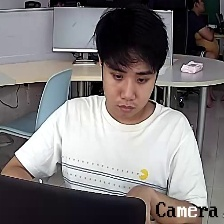
\includegraphics[width=\linewidth]{appendix/sit/000_CXS0_D0_005740.jpg}
    \end{subfigure}
    \begin{subfigure}[b]{0.45\linewidth}
      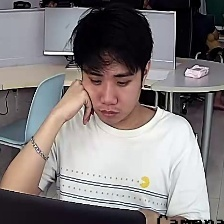
\includegraphics[width=\linewidth]{appendix/sit/000_CXS0_D0_006436.jpg}
    \end{subfigure}
    \begin{subfigure}[b]{0.45\linewidth}
      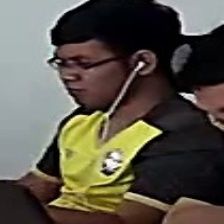
\includegraphics[width=\linewidth]{appendix/sit/000_CXS0_D0_005760.jpg}
    \end{subfigure}
    \begin{subfigure}[b]{0.45\linewidth}
      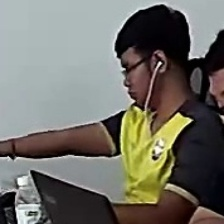
\includegraphics[width=\linewidth]{appendix/sit/000_CXS0_D0_006295.jpg}
    \end{subfigure}
    \caption{ตัวอย่างชุดข้อมูลในหมวดหมู่การกิน}
    \label{fig:result_track}
  \end{figure}

\clearpage
\subsection*{ตัวอย่างชุดข้อมูลสำหรับการสร้างโมเดลในหมวดหมู่ การนอน}
\begin{figure}[!ht]
    \centering
   \begin{subfigure}[b]{0.45\linewidth}
      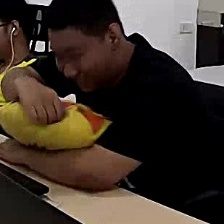
\includegraphics[width=\linewidth]{appendix/sleep/000_CXS0_D0_000043.jpg}
    \end{subfigure}
    \begin{subfigure}[b]{0.45\linewidth}
      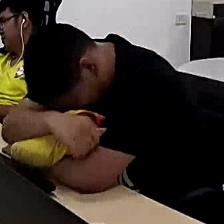
\includegraphics[width=\linewidth]{appendix/sleep/000_CXS0_D0_000052.jpg}
    \end{subfigure}
    \begin{subfigure}[b]{0.45\linewidth}
      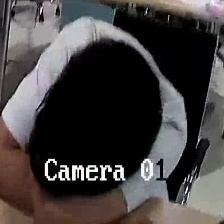
\includegraphics[width=\linewidth]{appendix/sleep/000_CXS0_D0_000069.jpg}
    \end{subfigure}
    \begin{subfigure}[b]{0.45\linewidth}
      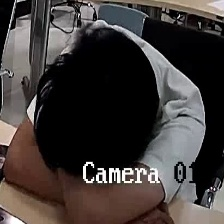
\includegraphics[width=\linewidth]{appendix/sleep/002_CXS0_D0_000782.jpg}
    \end{subfigure}
    \begin{subfigure}[b]{0.45\linewidth}
      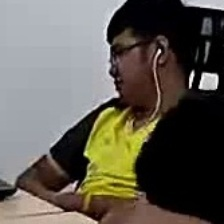
\includegraphics[width=\linewidth]{appendix/sleep/000_CXS0_D0_000073.jpg}
    \end{subfigure}
    \begin{subfigure}[b]{0.45\linewidth}
      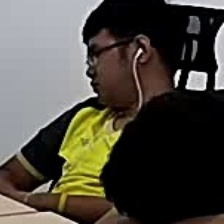
\includegraphics[width=\linewidth]{appendix/sleep/002_CXS0_D0_000647.jpg}
    \end{subfigure}
    \caption{ตัวอย่างชุดข้อมูลในหมวดหมู่การนอน}
    \label{fig:result_track}
  \end{figure}

\clearpage
\subsection*{ตัวอย่างชุดข้อมูลสำหรับการสร้างโมเดลในหมวดหมู่ การยืน}
\begin{figure}[!ht]
    \centering
   \begin{subfigure}[b]{0.45\linewidth}
      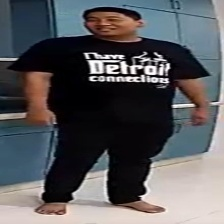
\includegraphics[width=\linewidth]{appendix/stand/000_CXS0_D0_001005.jpg}
    \end{subfigure}
    \begin{subfigure}[b]{0.45\linewidth}
      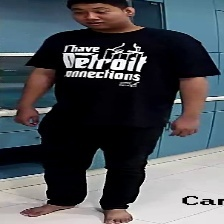
\includegraphics[width=\linewidth]{appendix/stand/000_CXS0_D0_001045.jpg}
    \end{subfigure}
    \begin{subfigure}[b]{0.45\linewidth}
      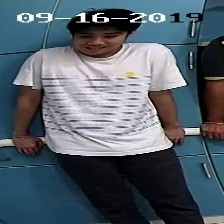
\includegraphics[width=\linewidth]{appendix/stand/000_CXS0_D0_001046.jpg}
    \end{subfigure}
    \begin{subfigure}[b]{0.45\linewidth}
      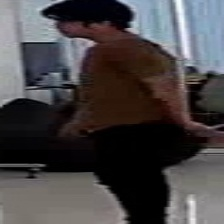
\includegraphics[width=\linewidth]{appendix/stand/001_CXS3_D2_000254.jpg}
    \end{subfigure}
    \begin{subfigure}[b]{0.45\linewidth}
      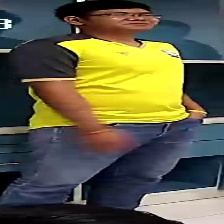
\includegraphics[width=\linewidth]{appendix/stand/000_CXS0_D0_000001.jpg}
    \end{subfigure}
    \begin{subfigure}[b]{0.45\linewidth}
      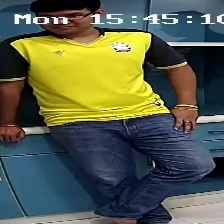
\includegraphics[width=\linewidth]{appendix/stand/000_CXS0_D0_000922.jpg}
    \end{subfigure}
    \caption{ตัวอย่างชุดข้อมูลในหมวดหมู่การยืน}
    \label{fig:result_track}
 \end{figure}


\clearpage
\subsection*{ตัวอย่างชุดข้อมูลสำหรับการสร้างโมเดลในหมวดหมู่ การเดิน}
\begin{figure}[!ht]
    \centering
    \begin{subfigure}[b]{0.45\linewidth}
      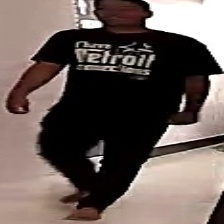
\includegraphics[width=\linewidth]{appendix/walk/000_CXS0_D0_000568.jpg}
    \end{subfigure}
    \begin{subfigure}[b]{0.45\linewidth}
      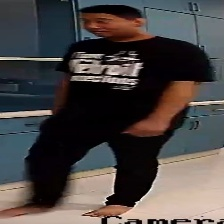
\includegraphics[width=\linewidth]{appendix/walk/000_CXS0_D0_0005656.jpg}
    \end{subfigure}
   \begin{subfigure}[b]{0.45\linewidth}
      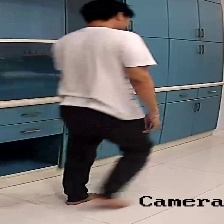
\includegraphics[width=\linewidth]{appendix/walk/000_CXS0_D0_000187.jpg}
    \end{subfigure}
    \begin{subfigure}[b]{0.45\linewidth}
      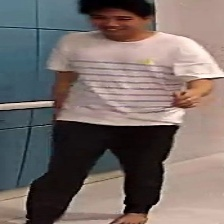
\includegraphics[width=\linewidth]{appendix/walk/000_CXS0_D0_000542.jpg}
    \end{subfigure}
    \begin{subfigure}[b]{0.45\linewidth}
      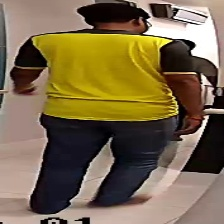
\includegraphics[width=\linewidth]{appendix/walk/000_CXS0_D0_000900.jpg}
    \end{subfigure}
    \begin{subfigure}[b]{0.45\linewidth}
      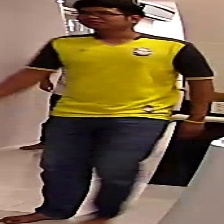
\includegraphics[width=\linewidth]{appendix/walk/000_CXS0_D0_000963.jpg}
    \end{subfigure}
    \caption{ตัวอย่างชุดข้อมูลในหมวดหมู่การยืน}
    \label{fig:result_track}
 \end{figure}

\clearpage
\subsection*{ตัวอย่างชุดข้อมูลสำหรับการสร้างโมเดลในหมวดหมู่รูปภาพทีเกิดข้อผิดพลาด}
รูปภาพที่เราคัดกรองออกเนื่องจากกกรณ๊พิเศษดังนี้ 1.มีบุคคลอยู่ไม่เต็มรูปภาพ 2.มีคนมากกว่า 1 คน ภายในรูปภาพ 3.รูปภาพมืดหรือไม่ชัด
\begin{figure}[!ht]
    \centering
    \begin{subfigure}[b]{0.45\linewidth}
      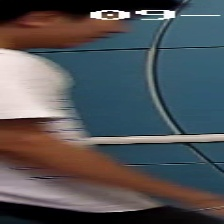
\includegraphics[width=\linewidth]{appendix/unknown/000_CXS0_D0_000149.jpg}
    \end{subfigure}
   \begin{subfigure}[b]{0.45\linewidth}
      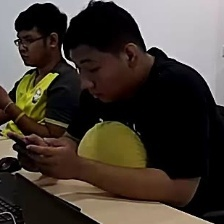
\includegraphics[width=\linewidth]{appendix/unknown/000_CXS0_D0_001793.jpg}
    \end{subfigure}
    \begin{subfigure}[b]{0.45\linewidth}
      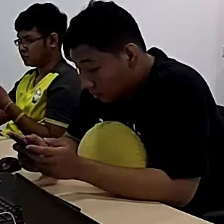
\includegraphics[width=\linewidth]{appendix/unknown/000_CXS0_D0_001794.jpg}
    \end{subfigure}
    \begin{subfigure}[b]{0.45\linewidth}
      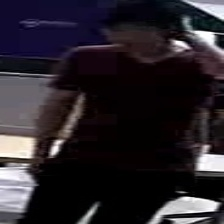
\includegraphics[width=\linewidth]{appendix/unknown/001_CXS2_D1_001979.jpg}
    \end{subfigure}
    \caption{ตัวอย่างชุดข้อมูลในหมวดหมู่รูปภาพทีเกิดข้อผิดพลาด}
    \label{fig:result_track}
 \end{figure}

